\documentclass[a4paper,12pt]{report}

\usepackage{pdfpages}
\usepackage{listofsymbols}
\usepackage{multirow}
\usepackage[pdftex]{hyperref}
\usepackage[dutch,english]{babel}
\usepackage{tikz}
%%\usepackage{mathdesign}
\usepackage{wrapfig}
%%\usepackage{picins} %plaatjes naast text
\usepackage{color}
\usepackage{enumerate}
%%\usepackage{enumitem}
\usepackage{paralist}
\usepackage{framed}
\usepackage{fancybox} %kaders

\usepackage{amsmath,amssymb,mathrsfs}
\usepackage{amsthm}
\usepackage{wasysym}
%\usepackage{extarrows}
\setlength{\parindent}{0pt}






\begin{document}

\section*{Grid Crossing}

\subsection*{Parameters}
For the Oedometer problem:

\begin{table}[h]
\centering
\begin{tabular}{l|l|l|l}
Quantity  & Symbol & Value  & Unit  \\ \cline{1-4}
   Density & $\rho$ & $1 \cdot 10^3$ & kg/m$^3$\\
   Young's modulus & E & $1 \cdot 10^5$ & Pa\\ 
Gravitational acc. & g & $-9.81$ & m/s$^2$ \\
Load & $p_0$ & $0$ & Pa \\
  Height  & H & $1$ & m \\ 
\end{tabular}
\end{table}

For the vibrating string with free end:

\begin{table}[h]
\centering
\begin{tabular}{l|l|l|l}
Quantity  & Symbol & Value  & Unit  \\ \cline{1-4}
   Density & $\rho$ & $1$ & kg/m$^3$\\
   Young's modulus & E & $100$ & Pa\\ 
Gravitational acc. & g & $0$ & m/s$^2$ \\
Load & $p_0$ & $0$ & Pa \\
  Height  & H & $25$ & m \\ 
\end{tabular}
\end{table}

For the test problem of Steffen et al.:

\begin{table}[h]
\centering
\begin{tabular}{l|l|l|l}
Quantity  & Symbol & Value  & Unit  \\ \cline{1-4}
   density & $\rho$ & $100$ & kg/m$^3$\\
   Young's modulus & E & $100$ & Pa\\ 
  length  & L & $1$ & m \\  
  amplitude force & $\tau$ & 1 & $-$\\
\end{tabular}
\end{table}

\newpage

\subsection*{Figure: internal force and pulse}
The figure was made with $10$ elements and $2$ PPC. A timestep was chosen of $\Delta t = 0.001$. \\
\\
As an alternative, we can also use the one I used during one of the meetings. (If you want, I will check the parameters/number of elements etc. for that figure.)

\subsection*{Figure: velocity}

\subsubsection*{Vibrating string with free end}
Two plots were made. The first one without grid crossing were we defined $30$ elements and $4$ PPC. The seconde one with grid crossing were we defined $60$ elements and $4$ PPC. In both cases a time step was used of $\Delta t = 0.01$ s. \\
\\
I think that these plots show nicely that grid crossing is a serious issue. (And that our code works)


\subsubsection*{Test problem Steffen et al.}
At this moment, there is no plot of the velocity implemented in the code (since it was not given in the paper). If you want I can implement it to obtain plots of the exact and obtained velocity. 

\subsubsection*{Oedometer problem}
Three plots were made. All of the plots were made with $30$ elements and $10$ PPC. A time step was used of $\Delta t = 0.001$ s. We have the following flavours:

\begin{itemize}
\item MPM solution and 'exact' solution.
\item MPM solution and ULFEM solution, both of node situated halfway.
\item MPM solution and ULFEM solution, MPM with particle situated halfway, ULFEM with node situated halfway.
\end{itemize}

\newpage 

\begin{center}
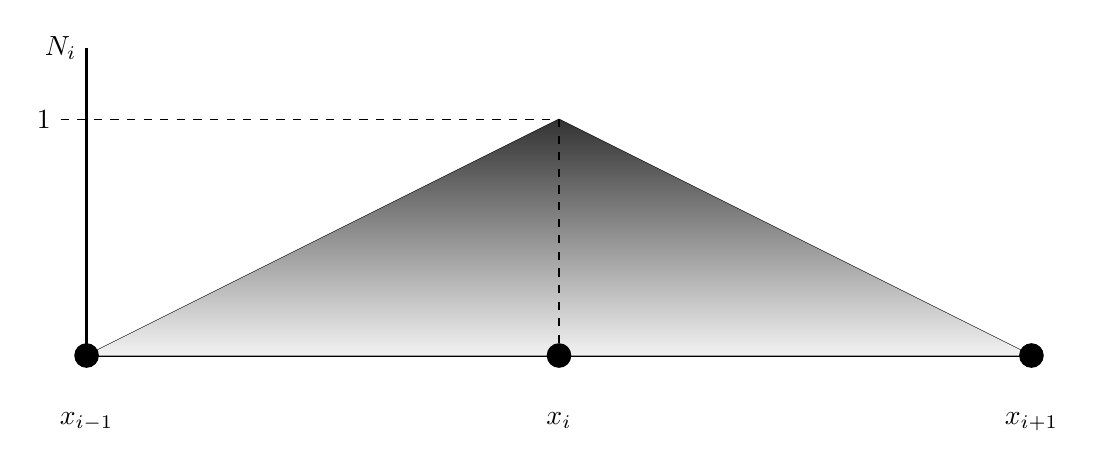
\begin{tikzpicture}[scale=3.0]
    % Draw axes
    \draw [-,thick] (0,1.3) node (yaxis) [left] {$N_i$}
        |- (4,0) node (xaxis) [right] {};
    % Draw two intersecting lines
    \draw (0,0) coordinate (a_1) -- (2,1) coordinate (a_2);
    \draw (2,1) coordinate (b_1) -- (4,0) coordinate (b_2);
    \draw (2,0) coordinate (b_3);
    \draw (0,-0.2) node[below] {$x_{i-1}$};
    \draw (2,-0.2) node[below] {$x_{i}$};
    \draw (4,-0.2) node[below] {$x_{i+1}$};
    
 \shade[bottom color=gray!10, top color=black!80] (0,0) --(2,0) --(2,1);
 \shade[bottom color=gray!10, top color=black!80] (4,0) --(2,0) --(2,1);

\node[draw,circle,inner sep=3pt,fill] at (b_3) {};
\node[draw,circle,inner sep=3pt,fill] at (b_2) {};
\node[draw,circle,inner sep=3pt,fill] at (a_1) {};

\draw[dashed] (yaxis |- b_1) node[left] {$1$}
        -| (xaxis -| b_1) node[below] {};

\end{tikzpicture}
\end{center}

\begin{center}
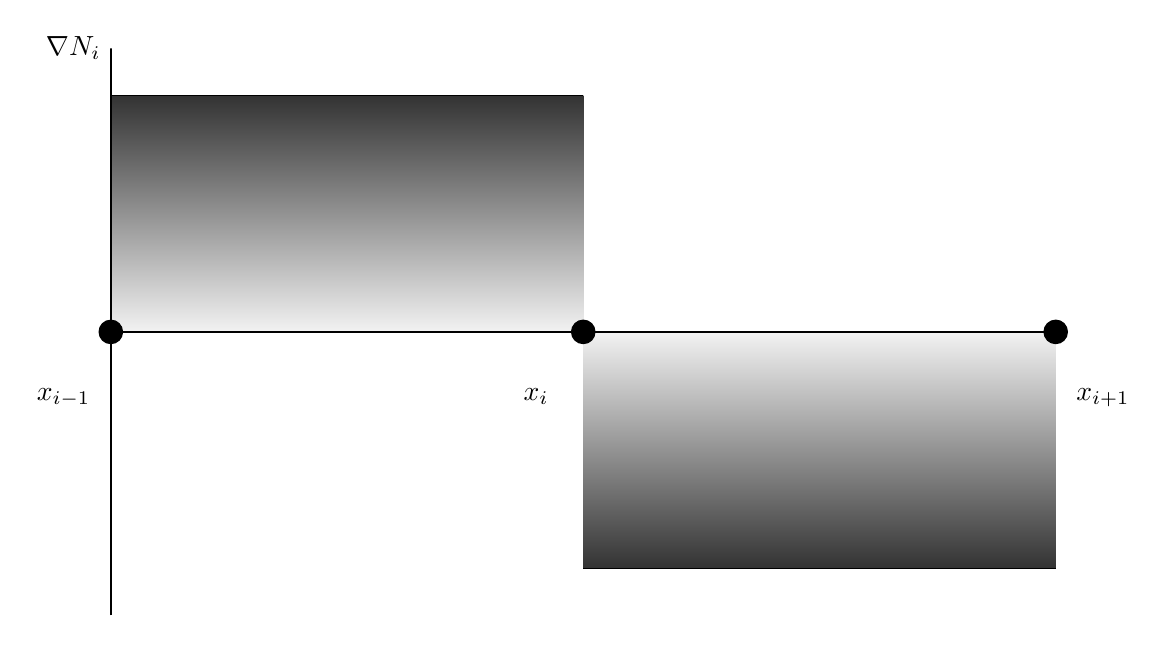
\begin{tikzpicture}[scale=3.0]
 \shade[bottom color=gray!10, top color=black!80] (0,0)rectangle +(2,1);
 \shade[top color=gray!10, bottom color=black!80] (2,0) rectangle +(2,-1);
    % Draw axes
    \draw [-,thick] (0,-1.2) -- (0,1.2) node (yaxis) [left] {$\nabla N_i$}
        |- (4,0) node (xaxis) [right] {};

    % Draw two intersecting lines
    \draw (0,1) coordinate (a_1) -- (2,1) coordinate (a_2);
    \draw (2,-1) coordinate (b_1) -- (4,-1) coordinate (b_2);
    \draw (2,0) coordinate (b_3);

    \draw (-0.2,-0.2) node[below] {$x_{i-1}$};
    \draw (1.8,-0.2) node[below] {$x_{i}$};
    \draw (4.2,-0.2) node[below] {$x_{i+1}$};
    


\node[draw,circle,inner sep=3pt,fill] at (0,0) {};
\node[draw,circle,inner sep=3pt,fill] at (2,0) {};
\node[draw,circle,inner sep=3pt,fill] at (4,0) {};


\end{tikzpicture}
\end{center}





\begin{center}
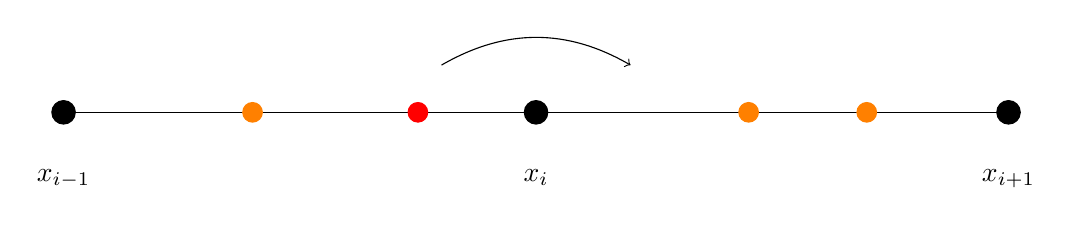
\begin{tikzpicture}[scale = 0.6]
\draw (0,0) coordinate(a_1) -- (10,0) coordinate(a_2);
\draw (a_1) -- (20,0) coordinate (a_3);

\draw (0,-1) coordinate (b_1);
\draw (20,-1) coordinate (b_3);
\draw (10,-1) coordinate (b_2);

\draw (b_1) node[below] {$x_{i-1}$};
\draw (b_3) node[below] {$x_{i+1}$} ;
\draw (b_2) node[below] {$x_{i}$};

\node[draw,circle,inner sep=3pt,fill] at (a_1) {};
\node[draw,circle,inner sep=3pt,fill] at (a_2) {};
\node[draw,circle,inner sep= 3pt,fill] at (a_3) {};

\node[draw,circle,inner sep=2.5pt,fill, color =orange] at (4,0) {};
\node[draw,circle,inner sep=2.5pt,fill, color = red] at (7.5,0) {};
\node[draw,circle,inner sep=2.5pt,fill, color =orange] at (14.5,0) {};
\node[draw,circle,inner sep=2.5pt,fill, color =orange] at (17,0) {};

 \draw[-to] (8,1) to[bend left] (12,1);

\end{tikzpicture}
\end{center}

\begin{center}
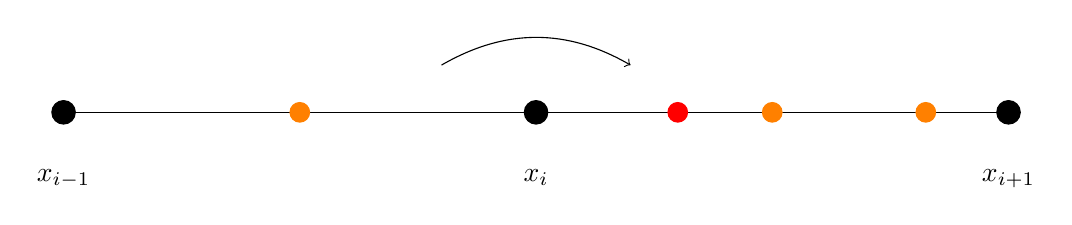
\begin{tikzpicture}[scale = 0.6]
\draw (0,0) coordinate(a_1) -- (10,0) coordinate(a_2);
\draw (a_1) -- (20,0) coordinate (a_3);

\draw (0,-1) coordinate (b_1);
\draw (20,-1) coordinate (b_3);
\draw (10,-1) coordinate (b_2);

\draw (b_1) node[below] {$x_{i-1}$};
\draw (b_3) node[below] {$x_{i+1}$} ;
\draw (b_2) node[below] {$x_{i}$};

\node[draw,circle,inner sep=3pt,fill] at (a_1) {};
\node[draw,circle,inner sep=3pt,fill] at (a_2) {};
\node[draw,circle,inner sep= 3pt,fill] at (a_3) {};

\node[draw,circle,inner sep=2.5pt,fill, color =orange] at (5,0) {};
\node[draw,circle,inner sep=2.5pt,fill, color = red] at (13,0) {};
\node[draw,circle,inner sep=2.5pt,fill, color =orange] at (15,0) {};
\node[draw,circle,inner sep=2.5pt,fill, color =orange] at (18.25,0) {};

 \draw[-to] (8,1) to[bend left] (12,1);

\end{tikzpicture}
\end{center}

\end{document}